% =====================================================================
% SLIDES DE APOIO (BACKUP) — fora da contagem principal, para arguição
% =====================================================================
\section*{Apêndice — Slides de Apoio}

%%% Backup B1 — Parametrização MIP-heurísticas
\begin{frame}{Apoio: parametrização das MIP-heurísticas}
    \begin{figure}
        \centering
        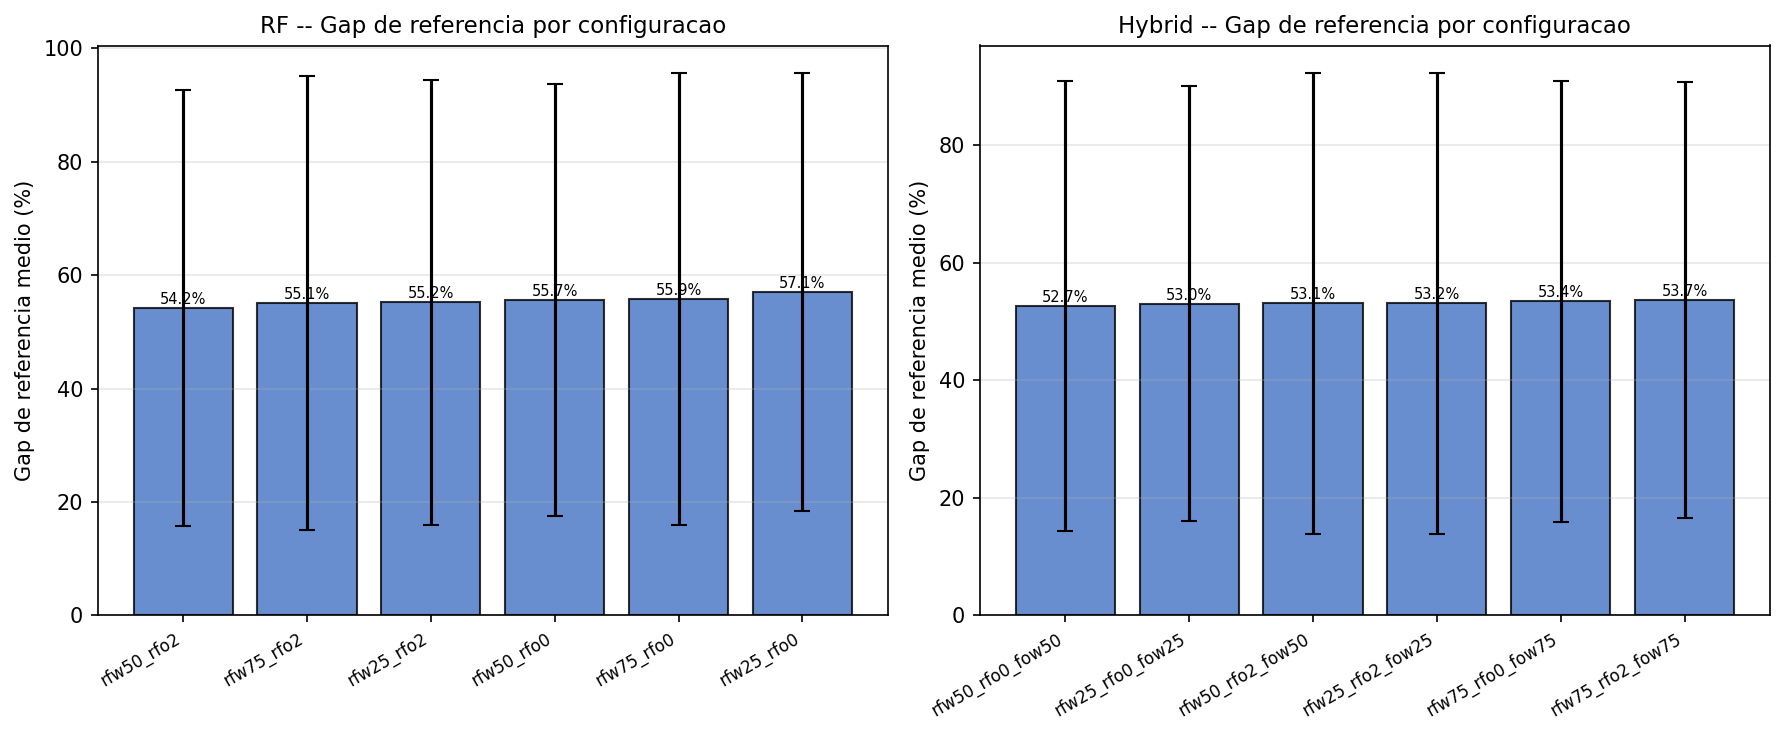
\includegraphics[width=0.95\linewidth]{img/param_mip_barchart.png}
        \caption{\textit{Gap} de referência por configuração de janela (15 dias).}
        \label{fig:bkp-param-mip}
    \end{figure}
    % TODO: RF w75/o2 e Híbrido w50/o2/w50 selecionados.
\end{frame}

%%% Backup B2 — Parametrização NSGA-II
\begin{frame}{Apoio: parametrização do NSGA-II}
    \begin{figure}
        \centering
        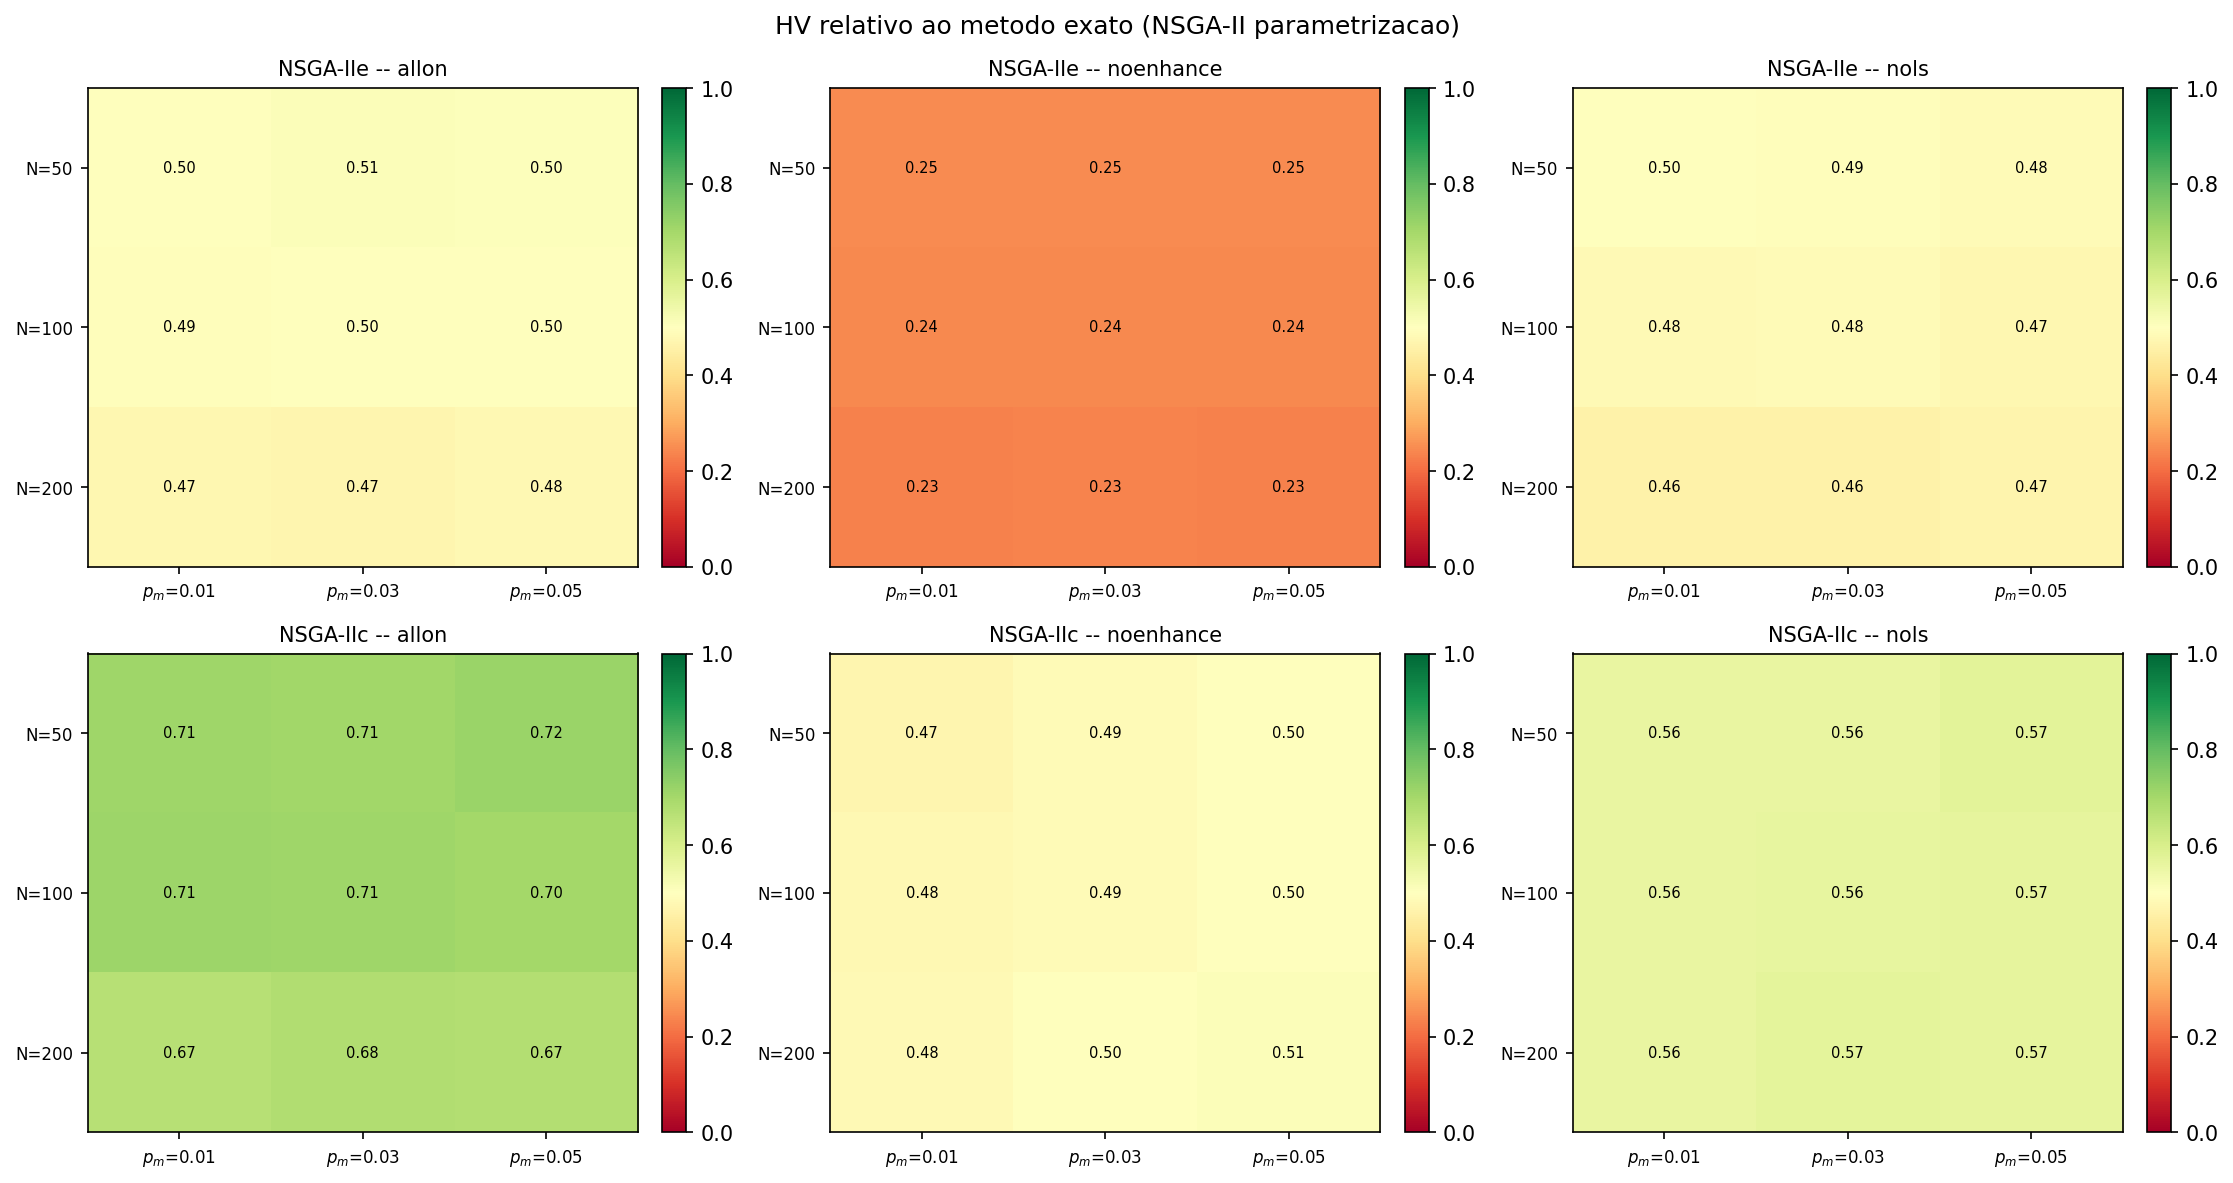
\includegraphics[width=\linewidth]{img/param_nsga2_heatmap.png}
        \caption{Hipervolume relativo por população/mutação (Compacto vs. Estendido).}
        \label{fig:bkp-param-nsga}
    \end{figure}
    % TODO: modo allon vence; Compacto HV rel. 0,67-0,72; Estendido 0,47-0,51.
\end{frame}

%%% Backup B3 — MIP gap por horizonte (heatmaps)
\begin{frame}{Apoio: MIP \textit{gap} por horizonte}
    \begin{columns}[c]
        \begin{column}{0.5\textwidth}
            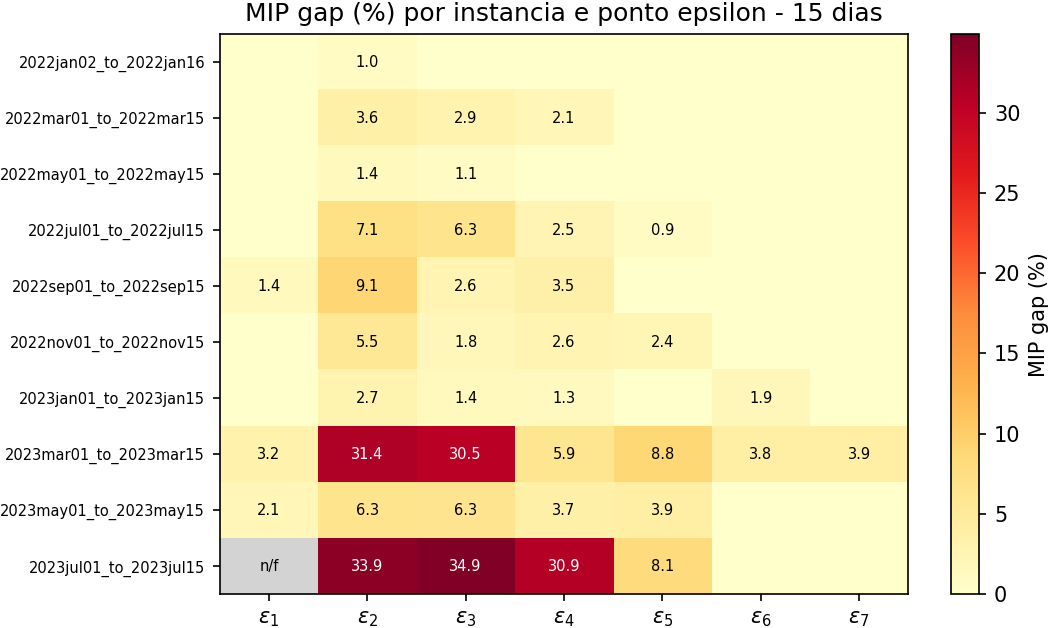
\includegraphics[width=\linewidth]{img/exato_mipgap_heatmap_15days.png}\\
            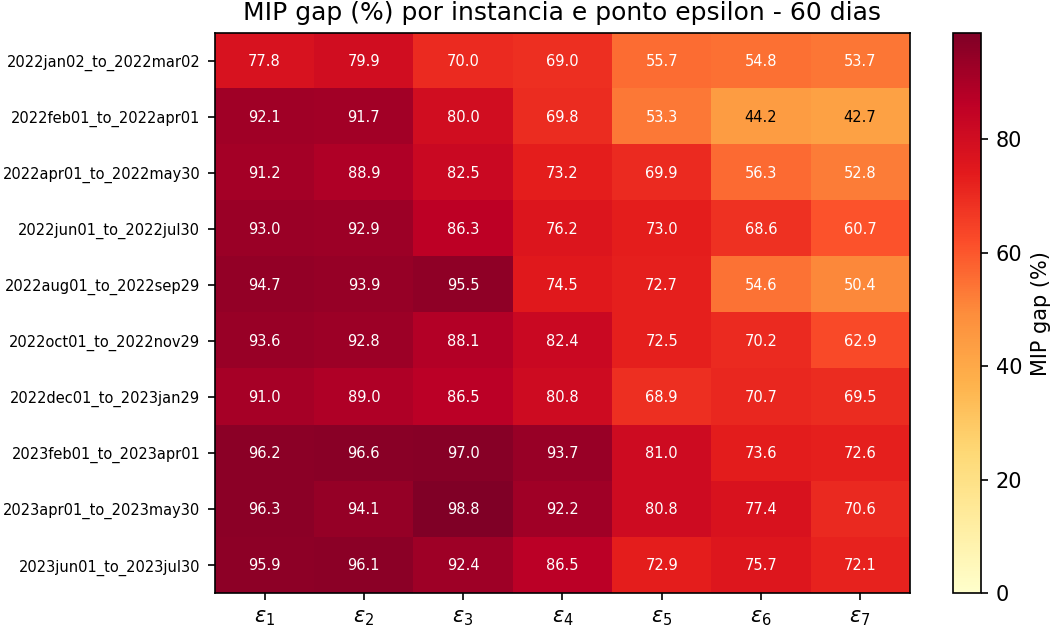
\includegraphics[width=\linewidth]{img/exato_mipgap_heatmap_60days.png}
        \end{column}
        \begin{column}{0.5\textwidth}
            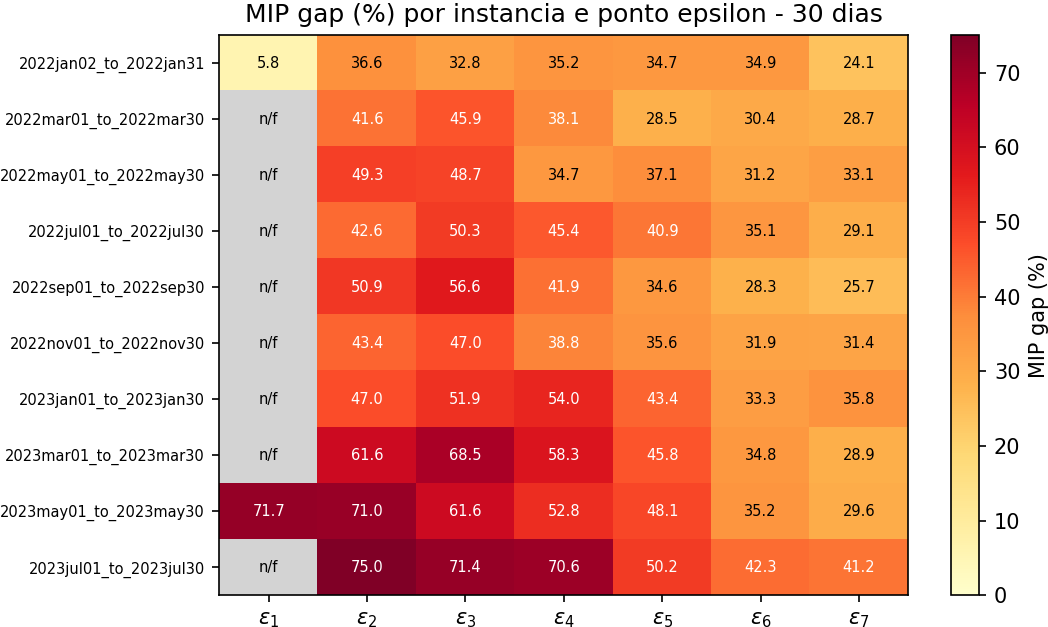
\includegraphics[width=\linewidth]{img/exato_mipgap_heatmap_30days.png}\\
            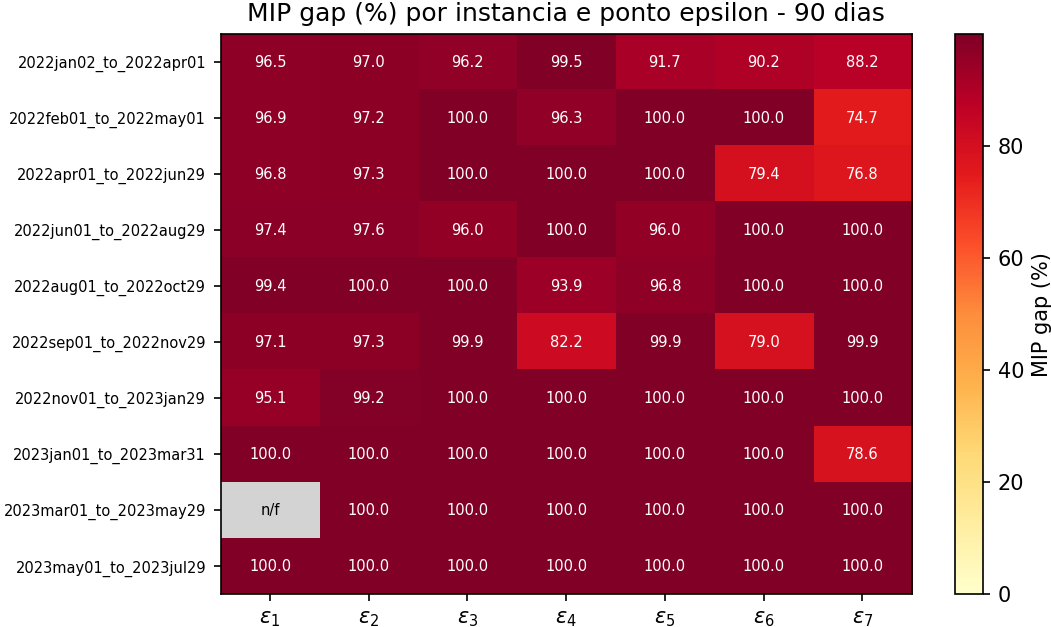
\includegraphics[width=\linewidth]{img/exato_mipgap_heatmap_90days.png}
        \end{column}
    \end{columns}
    % TODO: 15/30/60/90 dias.
\end{frame}

%%% Backup B4 — Tempo por horizonte (boxplots)
\begin{frame}{Apoio: tempo de execução por horizonte}
    \begin{columns}[c]
        \begin{column}{0.5\textwidth}
            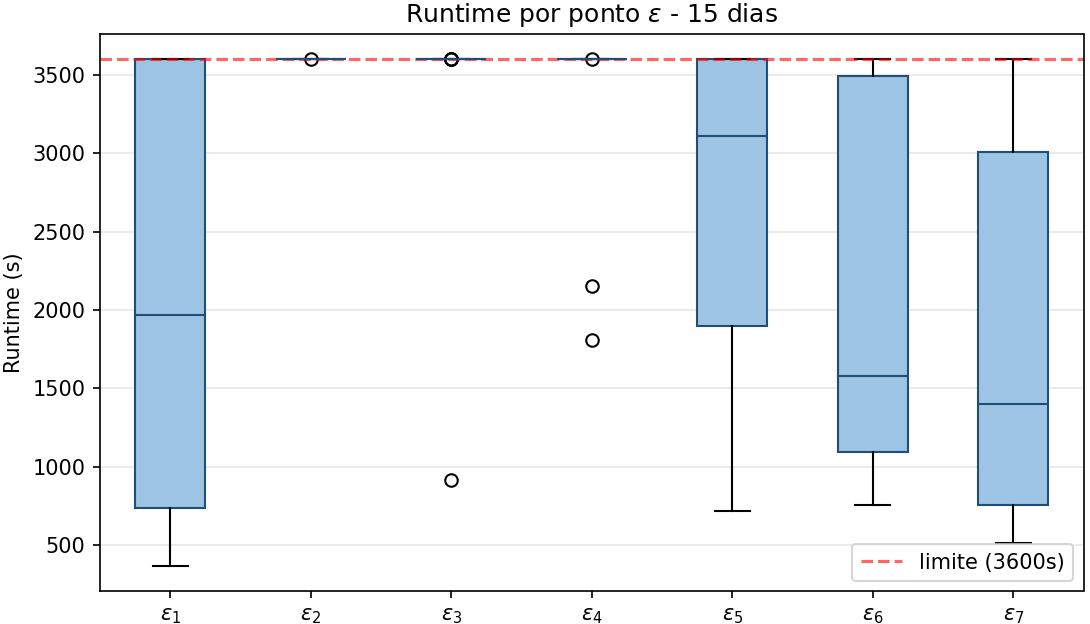
\includegraphics[width=\linewidth]{img/exato_runtime_boxplot_15days.png}\\
            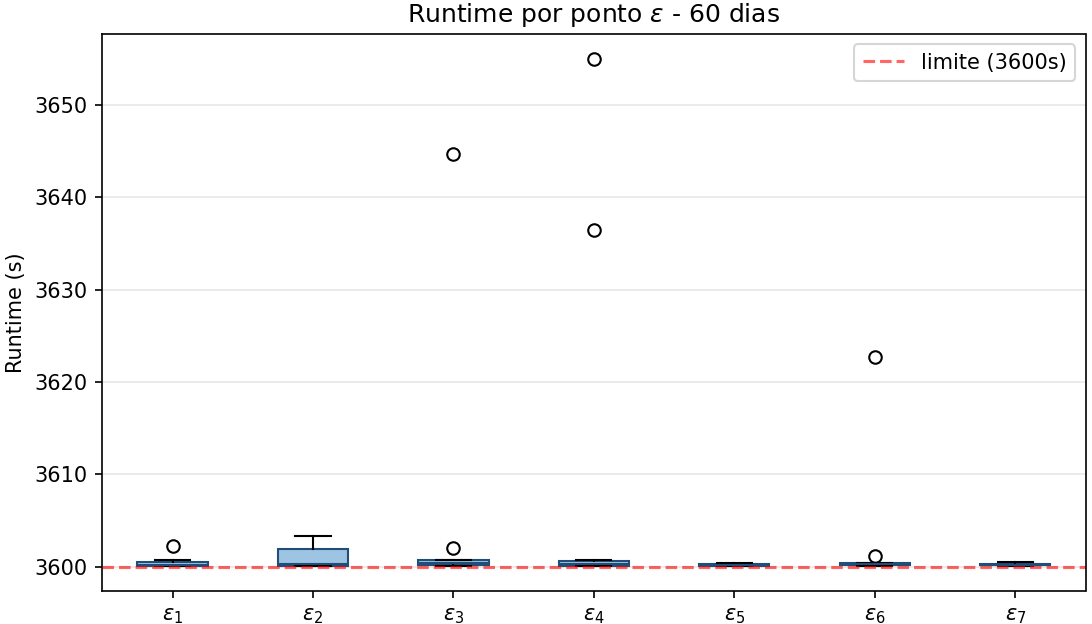
\includegraphics[width=\linewidth]{img/exato_runtime_boxplot_60days.png}
        \end{column}
        \begin{column}{0.5\textwidth}
            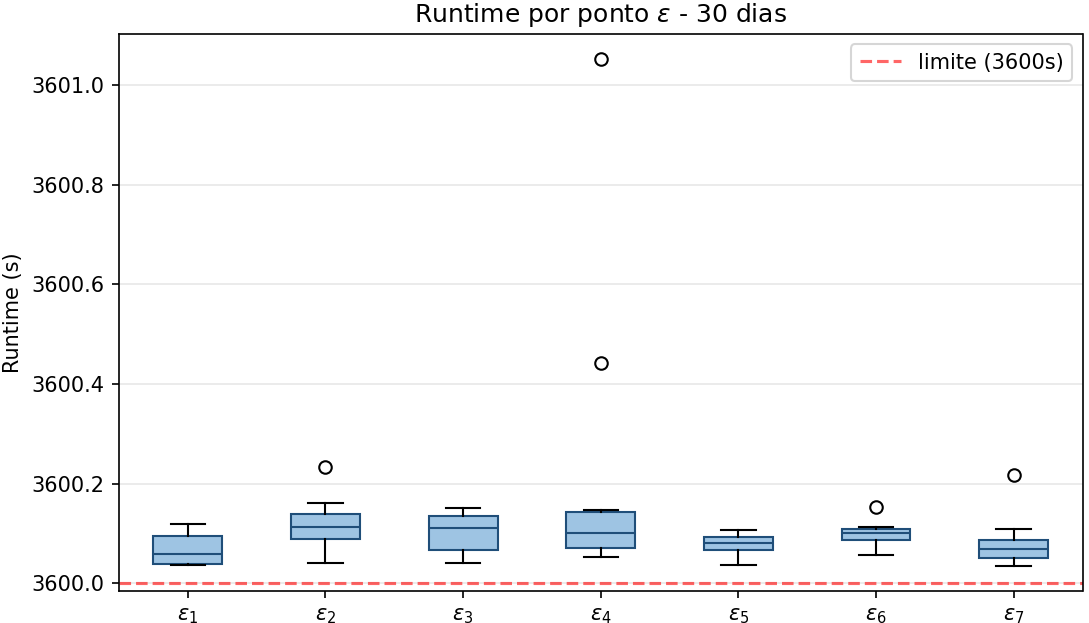
\includegraphics[width=\linewidth]{img/exato_runtime_boxplot_30days.png}\\
            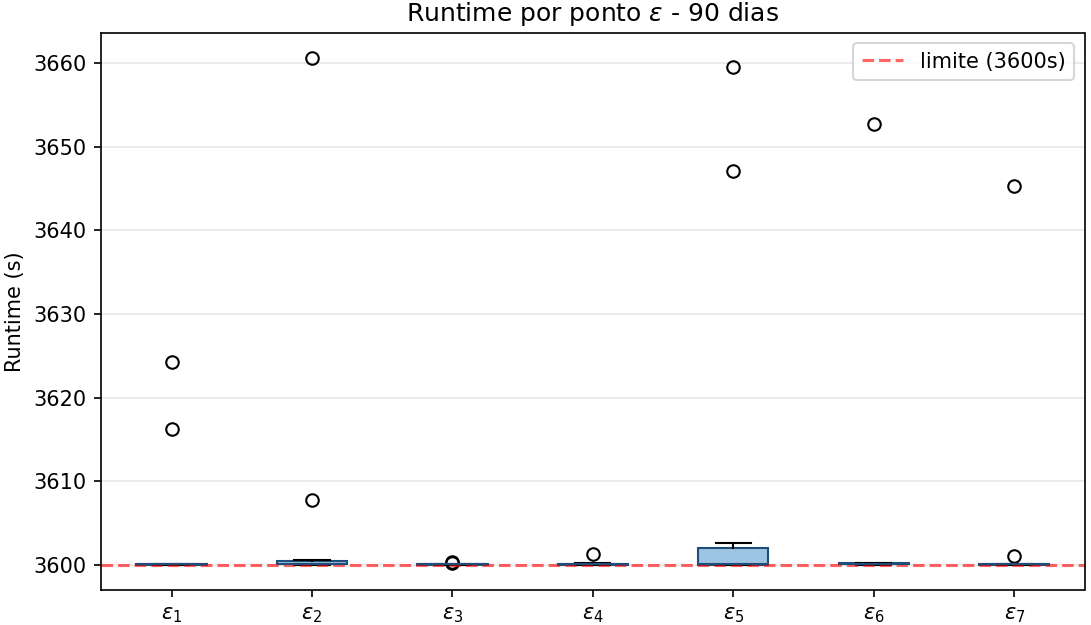
\includegraphics[width=\linewidth]{img/exato_runtime_boxplot_90days.png}
        \end{column}
    \end{columns}
\end{frame}

%%% Backup B5 — Estudo de caso (Gantt + ocupação)
\begin{frame}{Apoio: estudo de caso — agenda e ocupação}
    \begin{columns}[c]
        \begin{column}{0.5\textwidth}
            \begin{figure}
                \centering
                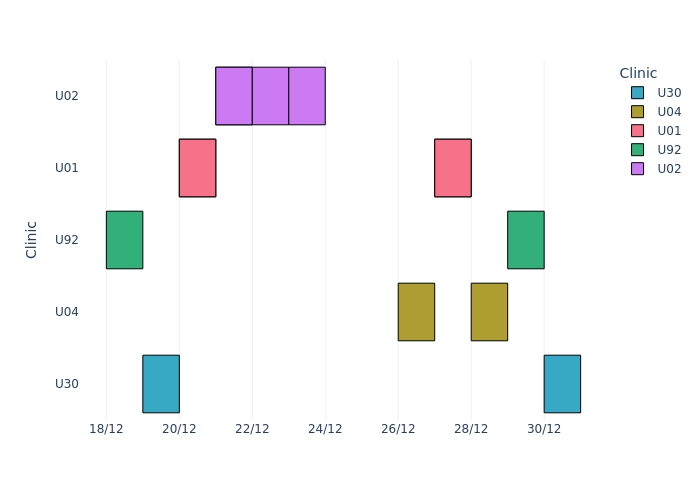
\includegraphics[height=3cm]{img/gantt_fo1.png}
                \caption{\footnotesize Agenda (extremo $Z_1$).}
            \end{figure}
        \end{column}
        \begin{column}{0.5\textwidth}
            \begin{figure}
                \centering
                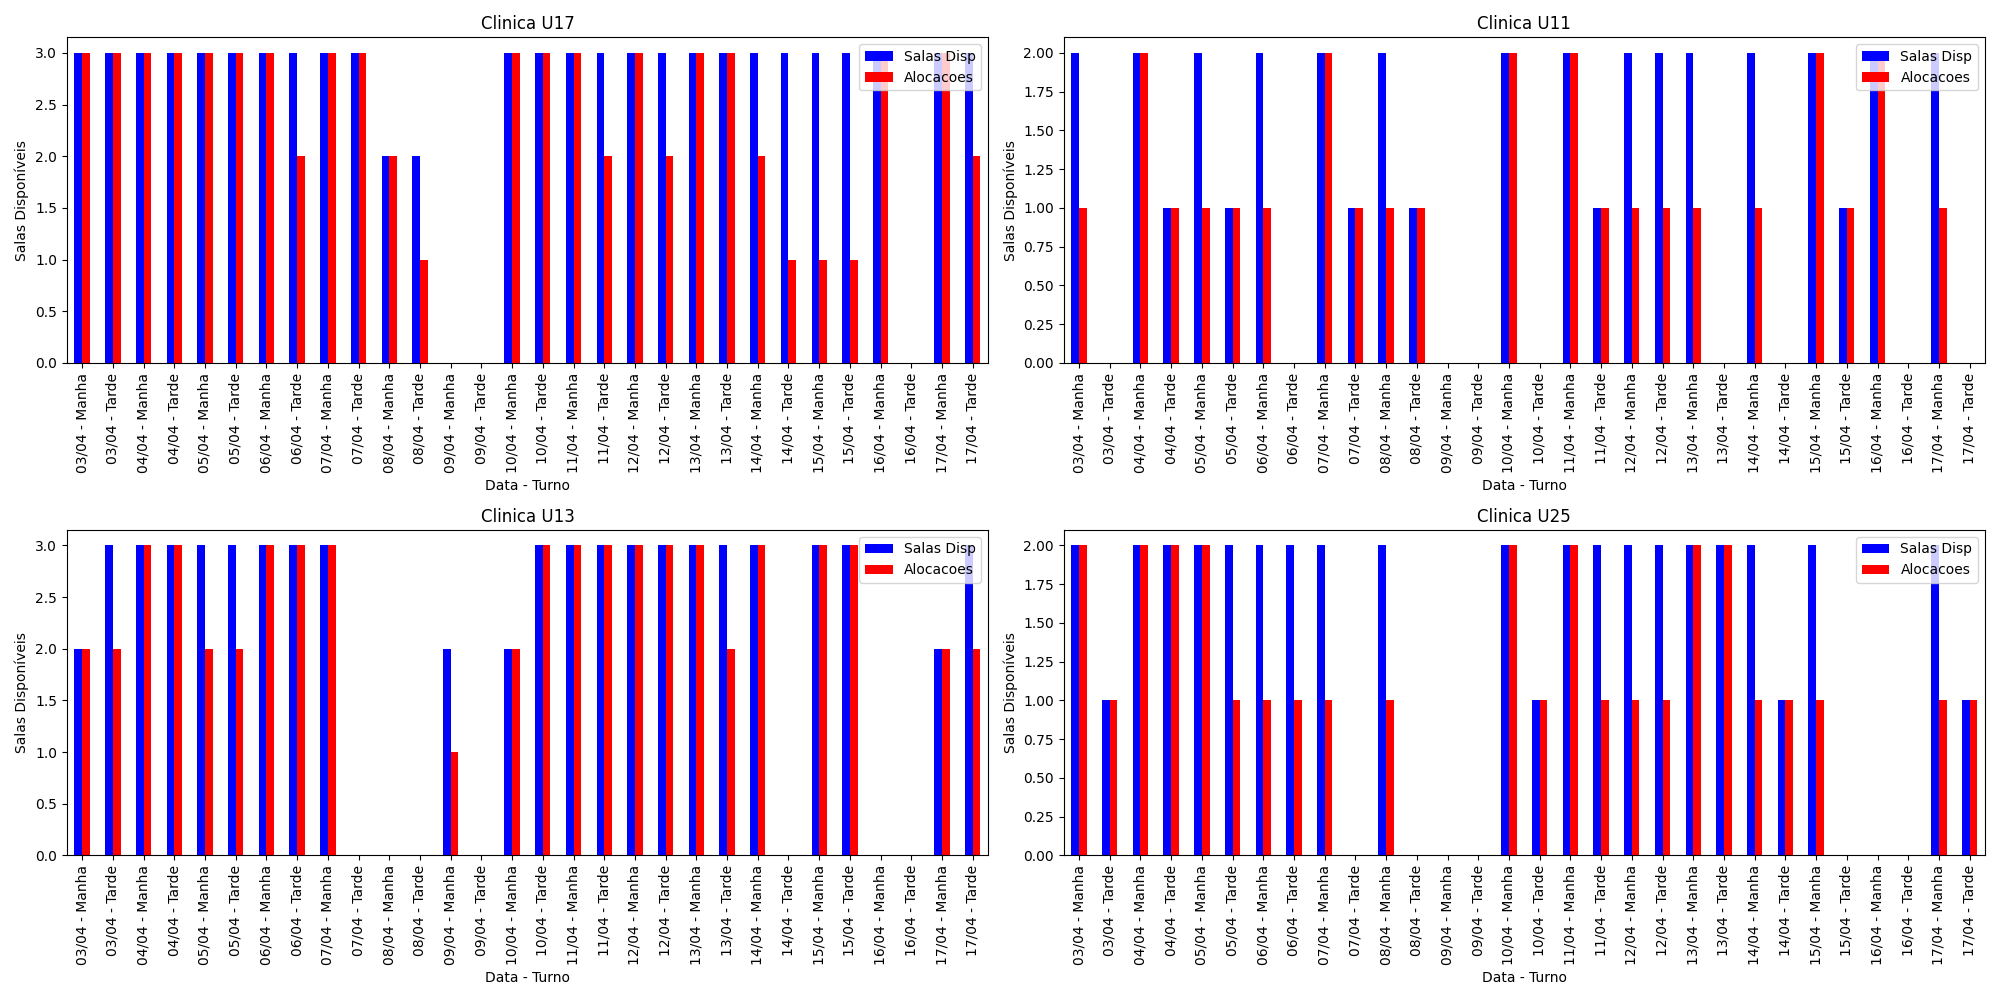
\includegraphics[height=3cm]{img/ocupacao_fo1.png}
                \caption{\footnotesize Ocupação de salas.}
            \end{figure}
        \end{column}
    \end{columns}
    % TODO: alternar entre gantt_fo1/fo2/fo3 e ocupacao_fo* conforme a pergunta.
\end{frame}
